%% Copernicus Publications Manuscript Preparation Template for LaTeX Submissions
%% ---------------------------------
%% This template should be used for copernicus.cls
%% The class file and some style files are bundled in the Copernicus Latex Package, which can be downloaded from the different journal webpages.
%% For further assistance please contact Copernicus Publications at: production@copernicus.org
%% https://publications.copernicus.org/for_authors/manuscript_preparation.html


%% Please use the following documentclass and journal abbreviations for preprints and final revised papers.

%% 2-column papers and preprints
\documentclass[gmd, manuscript]{copernicus}



%% Journal abbreviations (please use the same for preprints and final revised papers)


% Advances in Geosciences (adgeo)
% Advances in Radio Science (ars)
% Advances in Science and Research (asr)
% Advances in Statistical Climatology, Meteorology and Oceanography (ascmo)
% Aerosol Research (ar)
% Annales Geophysicae (angeo)
% Archives Animal Breeding (aab)
% Atmospheric Chemistry and Physics (acp)
% Atmospheric Measurement Techniques (amt)
% Biogeosciences (bg)
% Climate of the Past (cp)
% DEUQUA Special Publications (deuquasp)
% Earth Surface Dynamics (esurf)
% Earth System Dynamics (esd)
% Earth System Science Data (essd)
% E&G Quaternary Science Journal (egqsj)
% EGUsphere (egusphere) | This is only for EGUsphere preprints submitted without relation to an EGU journal.
% European Journal of Mineralogy (ejm)
% Fossil Record (fr)
% Geochronology (gchron)
% Geographica Helvetica (gh)
% Geoscience Communication (gc)
% Geoscientific Instrumentation, Methods and Data Systems (gi)
% Geoscientific Model Development (gmd)
% History of Geo- and Space Sciences (hgss)
% Hydrology and Earth System Sciences (hess)
% Journal of Bone and Joint Infection (jbji)
% Journal of Micropalaeontology (jm)
% Journal of Sensors and Sensor Systems (jsss)
% Magnetic Resonance (mr)
% Mechanical Sciences (ms)
% Natural Hazards and Earth System Sciences (nhess)
% Nonlinear Processes in Geophysics (npg)
% Ocean Science (os)
% Polarforschung - Journal of the German Society for Polar Research (polf)
% Primate Biology (pb)
% Proceedings of the International Association of Hydrological Sciences (piahs)
% Safety of Nuclear Waste Disposal (sand)
% Scientific Drilling (sd)
% SOIL (soil)
% Solid Earth (se)
% State of the Planet (sp)
% The Cryosphere (tc)
% Weather and Climate Dynamics (wcd)
% Web Ecology (we)
% Wind Energy Science (wes)


%% \usepackage commands included in the copernicus.cls:
%\usepackage[german, english]{babel}
%\usepackage{tabularx}
%\usepackage{cancel}
%\usepackage{multirow}
%\usepackage{supertabular}
%\usepackage{algorithmic}
%\usepackage{algorithm}
%\usepackage{amsthm}
%\usepackage{float}
%\usepackage{subfig}
%\usepackage{rotating}
\usepackage{booktabs}

\newcommand{\dd}{\mathrm{d}}

\begin{document}

\title{An information-theoretic approach to obtain ensemble averages from Earth system models}


% \Author[affil]{given_name}{surname}

\Author[1][csierra@bgc-jena.mpg.de]{Carlos A.}{Sierra} %% correspondence author
\Author[1,2]{Estefanía}{Muñoz}

\affil[1]{Max Planck Institute for Biogeochemistry, Jena, Germany}
\affil[2]{CREAF, Cerdanyola del Vallès, Barcelona, Spain}

%% The [] brackets identify the author with the corresponding affiliation. 1, 2, 3, etc. should be inserted.

%% If an author is deceased, please mark the respective author name(s) with a dagger, e.g. "\Author[2,$\dag$]{Anton}{Smith}", and add a further "\affil[$\dag$]{deceased, 1 July 2019}".

%% If authors contributed equally, please mark the respective author names with an asterisk, e.g. "\Author[2,*]{Anton}{Smith}" and "\Author[3,*]{Bradley}{Miller}" and add a further affiliation: "\affil[*]{These authors contributed equally to this work.}".


\runningtitle{TEXT}

\runningauthor{Sierra \& Muñoz}





\received{}
\pubdiscuss{} %% only important for two-stage journals
\revised{}
\accepted{}
\published{}

%% These dates will be inserted by Copernicus Publications during the typesetting process.


\firstpage{1}

\maketitle



\begin{abstract}
Inferences in Earth system science rely to a large degree on the numerical output of multiple Earth System Models. It has been shown that for many variables of interest, the multi-model ensemble average often compares better with observations than the output from any one individual model. However, a simple arithmetic average does not reward or penalize models according to their ability to predict available observations, and for this reason, a weighted averaging approach would be preferred for those cases in which there is information on model performance. We propose an approach based on concepts from information theory with the aim to approximate the Kullback-Leibler distance between model output and unknown reality, and to assign weights to different models according to their relative likelihood of being the best-performing model in a given grid cell. This article presents the theory and describes the steps necessary for obtaining model weights in a general form, and presents an example for obtaining multi-model averages of carbon fluxes from models participating in the sixth phase of the Coupled Model Intercomparison Project CMIP6. Using this approach, we propose a multi-model ensemble of land-atmosphere carbon exchange that could be used for inferring long-term carbon balances with much reduced uncertainties in comparison to the multi-model arithmetic average. 
\end{abstract}


%\copyrightstatement{TEXT} %% This section is optional and can be used for copyright transfers.


\introduction  %% \introduction[modified heading if necessary]
Inferences in Earth system science (ESS) depend to a large extent on the output from Earth system models (ESMs) that combine different components of the carbon, water, and energy balance of Earth and make spatial and temporal predictions of a large number of variables of scientific interest. These models are relatively large and transcend specific knowledge of single disciplines. Multiple modeling groups run large simulations and participate in coordinated Model Intercomparison Projects (MIP), where the forcings to the model are similar and the outputs across models are comparable \citep{Eyring2016}. For making inferences about a particular aspect of the dynamics of the Earth system, one is confronted with the problem of what model to analyze, how to assign a degree of belief to the results of a certain model, and how to perform averaging across models to obtain an unbiased estimator of some variable of interest \citep{Hagedorn2005, Knutti2010CC, Knutti2010JC, Hausfather2022, Tebaldi2007}. 

These problems are not new to science, and a lot of previous work has been done in the fields of information theory and statistics to address some of these issues. In particular, the problem of model selection and multi-model inference in statistics, where the idea is to fit multiple models to observed data, is relatively well developed \citep{Anderson2007, Burnham2002, Millington2011, Claeskens2008}. However, classical multi-model inference methods have been developed mostly for simple statistical models, usually expressed as polynomial functions, and not for dynamical models that recursively update a large set of state variables based on a dynamical rule as in ESMs. Therefore, there is a need to expand the existing theory of multi-model inference to the large-dimensional models used in Earth system science.

Three main challenges emerge when trying to expand statistical methods of multi-model inference to ESMs. First, ESMs are not parameterized using statistical techniques such as maximum likelihood estimation (MLE) for the entire set of parameters of the model, which may vary spatially depending on the process being represented. Hirotugu Akaike showed in his seminal work that a measure of distance among models can be obtained with the log-likelihood estimate of the model with respect to an observational set \citep{Akaike1974, Akaike1981}. Thus, the challenge is to find a way to obtain a distance metric that does not rely on MLE methods. This is particularly important for ESMs because model uncertainty not only includes parameter uncertainty but also uncertainty due to initial states and boundary conditions \citep{Tebaldi2007}.
A second challenge is that the total number of parameters in a given ESM is usually unknown to the user of ESM numerical output. The classical statistical theory assigns penalties to models according to their number of parameters, but this is practically impossible for published output from ESMs because there is no consistent reporting of the type and number of parameters, and whether they were obtained by an optimization method or agnostically inputted. Thus, the classical theory needs to be modified by an approach that disregards model complexity and does not add a penalty for it. 
A third challenge is the high-dimensionality of the problem of multi-model inference with ESMs. While the classical theory usually considers one predicted variable and a small set of explanatory variables linked by a polynomial function, the problem in ESS is to obtain expected values of a large set of state variables reported in a multi-dimensional lattice (geographical coordinates, time, and height or depth). 

In this article, we propose an adaptation of the classical statistical theory of multi-model inference addressing the challenges of lack of MLE, unknown parameter space, and high dimensionality. We explicitly deal with the problem of model averaging following the conceptual approach described by \citet{Burnham2002}, which builds on the work developed by H. Akaike in the 1970s and 80s \citep{Parzen1998}.

It has been shown in previous publications that the multi-model average of a variable of interest such as surface air temperature tends to agree better with observations than the predictions of any one single model \citep{Doblas-Reyes2003, Hagedorn2005, Elvidge2023}. The arithmetic mean from a set of models gives no consideration about the ability of some models to perform better than others. This is equivalent to assuming that each model is weighted equally in their prediction ability. However, it has been shown that this `model democracy' is inappropriate for multi-model inference in climate science \citep{Knutti2010CC, Knutti2017}. Although we are aware that other approaches for multi-model averaging of ESM output have been proposed before \citep[e.g.,][]{Knutti2017, Ribes2021, Sanderson2015, Giorgi2002, Tebaldi2007, Tebaldi2005, Elvidge2023}, we are not aware of a previous methodology grounded on information-theoretic principles. In addition, some previous approaches calculate weights as fixed values for all output of a model, but it is desirable to obtain weights based on the ability of some models to provide better estimates for some spatial regions than others. Our proposed approach operates at the grid-cell level and, therefore, produces weights based on the ability of a model to predict the spatial distribution of a variable of interest.

This article is organized as follows, first, we provide a conceptual derivation of a distance metric appropriate for ESMs using classical concepts from multi-model inference, and a derivation of model weights to obtain ensemble averages and uncertainties. The conceptual framework presented here follows the derivation presented by \citet{Burnham2002}, but adapted to the specific case of ESMs. Then, we present a step-by-step description of the method applied to multidimensional ESM numerical output. We later apply the method to the computation of the average net carbon exchange between the land and the atmosphere using models from the CMIP6 archive and discuss the results. 

\section{Conceptual approach}
We assume that a model $g$ is an approximation of the unknown full reality $f$, and the \emph{distance} between $g$ and $f$ is given by the Kullback-Liebler information
\begin{equation} \label{eq:KLD}
I(f, g) = \int f(x) \log \left( \frac{f(x)}{g(x | \theta)} \right) \dd x,
\end{equation}
where $x$ is the variable being modeled, and $\theta$ is the set of parameters in the model $g$. 
In this framework, both $f$ and $g$ are understood as probability density functions. In the case of ESM model output, we can think of them as the proportional distribution of some quantity $x$ over a spatial and temporal domain. 
For ESMs, the vector $\theta$ not only includes the set of parameters in the model, but also the set of initial conditions for the state variables that may lead to different ESM outputs. 

This distance $I(f, g)$ can be interpreted as the loss of information from full reality by the model. In principle, we are interested in selecting or ranking models according to $I(f, g)$, but in practice, we cannot compute $f(x)$. 
This limitation is partly alleviated, as we will see later, by the expansion of equation~\ref{eq:KLD} as
\begin{equation} \label{eq:KLD_expan}
I(f, g) = \int f(x) \log f(x) \dd x - \int f(x) \log (g(x | \theta)) \dd x.
\end{equation}
Notice that each of these terms on the rhs of equation \ref{eq:KLD_expan} can be considered as an expectation of a probability distribution. Furthermore, because full reality $f$ is a fixed quantity that does not depend on parameters or initial conditions, the first term on the rhs of \ref{eq:KLD_expan} can be considered as a constant. In terms of expectations, equation~\ref{eq:KLD_expan} can be written as
\begin{equation}\label{eq:KLD_expect}
I(f, g)  = E_f[ \log(f(x)) ] - E_f [ \log (g(x | \theta)) ].
\end{equation}
This equation suggests that for a given model $g$, there would be a set $\theta_m$ that minimizes the distance from reality $f$. 

In the process of model development, investigators often make decisions about initial and boundary conditions, and the proper parameterization of the model based on previous knowledge and certain data $y$ that they have at hand. A model would have a set of estimated parameters depending on the available data, which can be expressed as $\hat{\theta} (y)$. It is reasonable to expect that the set $\hat{\theta}$ does not correspond to $\theta_m$, and in fact, in most cases, the configuration of a model would be further apart from the configuration that would minimize its distance to full reality. 

In terms of expectations, we are then interested in obtaining an estimator of the distance $I(f, g)$ with respect to the variable of interest $x$ and the available data $y$, expressed as
\begin{equation}
E_y \ E_x [\log(g(x | \hat{\theta}(y) ))].
\end{equation}

The seminal work of H. Akaike showed that this expectation can be approximated by the log-likelihood function of the fitted parameters given the data
\begin{equation}
\log (\mathcal{L}(\hat{\theta} | y) ) \approx E_y \ E_x [\log(g(x | \hat{\theta}(y) ))],
\end{equation}
which is equivalent to
\begin{equation}
\log (\mathcal{L}(\hat{\theta} | y) ) \approx \hat{E}_{\hat{\theta}} [I(f, \hat{g})],
\end{equation}
where the $\approx$ symbol is used here instead of an equality because a bias-correction term $K$ (number of parameters in the model) used by Akaike is ignored in this expression. The key result is that the log-likelihood of a model, configured with parameters and initial conditions consistent with some observed data, is an approximation of its expected distance to full reality.

The non-trivial problem now is to determine a reasonable value of a log-likelihood for a parameterized ESM given some observed data. In contrast to common statistical methods of maximum likelihood estimation (MLE) for simple statistical models, there is not (to our knowledge) any method for MLE dealing with the hundreds of parameters in an ESM. Also, there is not really any observed data on the gridded format required for comparison with ESM output because measurements are not performed systematically for all points on the surface of the Earth. What we usually have available is data products that are derived from sparse observations and scaled to the terrestrial surface following some data manipulation technique. 

Under strong assumptions of linearity, equal variance, and probability distributions from the exponential family (normal, exponential), least-square estimates are identical to maximum likelihood estimates. This is surely not the case for the distribution of output variables from ESMs, but given the absence of any other method for obtaining a log-likelihood function of a parameterized ESM with respect to data, we make here the strong assumption that
\begin{equation} \label{assumption}
n \log(\hat{\sigma}^2) \approx \log (\mathcal{L}(\hat{\theta} | y) ),
\end{equation}
where 
\begin{equation}
\hat{\sigma}^2 = \frac{\sum^n \hat{\epsilon}_j^2 }{n},
\end{equation}
and $\hat{\epsilon}$ are residuals between model predictions and some available data product. The lhs in equation~\ref{assumption} is the first component of Akaike's Information Criterion (AIC) for the least-squares case without the correction term $K$. Although not perfect, this approximation to the AIC and the log-likelihood function can be estimated from existing model output from ESMs and some observational data product, provided that both are available for the same spatial and temporal coordinates. Thus, mimicking the definition of AIC, we define for our purposes the distance metric $\mathcal{A}$ as

\begin{equation}
\mathcal{A} := n \log (\hat{\sigma}^2).
\end{equation} 

One characteristic of $\mathcal{A}$ is that it preserves some of the properties of AIC; it can be viewed as a negative entropy \citep{Akaike1985}, and can be used to compare its value across different models on an absolute scale. In other words, one can compute $\mathcal{A}_i$ for a set of models $i \in [1, \dots ,k]$ and rank them according to their relative difference. One of the models in the set would have the minimum value $\mathcal{A}_m$ and can be considered as the model with the minimum distance to the observations. Furthermore, for any other model in the set, we can calculate their difference with respect to this `best' model as
\begin{equation}
\Delta_i := \mathcal{A}_i - \mathcal{A}_m.
\end{equation}
More importantly, the values of $\Delta_i$ are estimates of 
\begin{equation}
E_{\hat{\theta}} [\hat{I}(f, g_i)] - \min E_{\hat{\theta}} [\hat{I}(f, g_i)],
\end{equation}
i.e., they are estimates of the relative difference between the expected distance between the model and full reality with respect to the same distance for the model that is closer to full reality (Figure~\ref{fig:concept}). Recall from equation~\ref{eq:KLD_expect} that the expected value for full reality is a constant, therefore its actual value plays no role regarding these values of $\Delta_i$.

\begin{figure}[ht]
   \centering
   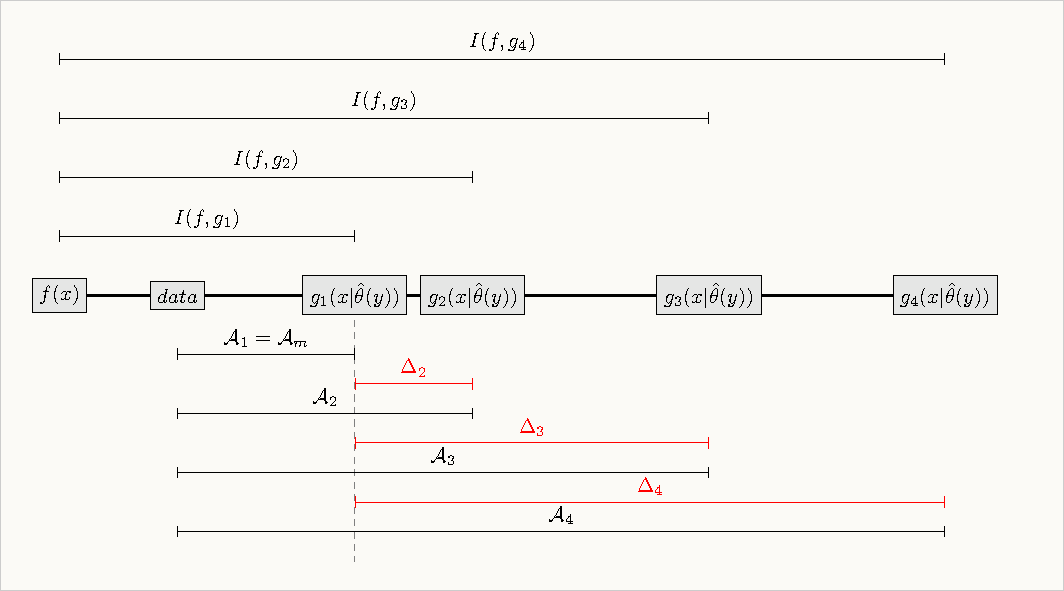
\includegraphics[width=14cm]{Figures/distances.pdf} % requires the graphicx package
   \caption{Conceptual representation of the approximation of the Kullback-Liebler distance between models and full reality $I(f, g_i)$ by the proposed metric $\mathcal{A}_i$, and relative ranking of models according to the metric $\Delta_i$. Models $g_i$ predict the value of variable $x$ based on a configuration of parameters and initial conditions encoded in the vector $\hat{\theta}$, which is based on some a priori data $y$. In this example, the model with the closest distance to the reference data is $g_1$, so $\mathcal{A}_1 = \mathcal{A}_m$. The relative ranking among models is defined as $\Delta_i = \mathcal{A}_i - \mathcal{A}_m$. Notice that the distance from full reality and data is always constant as well as the distance from full reality to model $g_1$. Therefore, the relative ranking of the models is similar to ranking models based on their Kullback-Liebler distance to full reality.}
   \label{fig:concept}
\end{figure}

Another important contribution of H. Akaike is a method to obtain the likelihood of a model given the data $\mathcal{L}(g_i | data)$ based on the value of $\Delta_i$ for each model. It can be interpreted as the relative strength of evidence for a particular model in the set of models being considered given the available data, and it is expressed as
\begin{equation}
\mathcal{L}(g_i | data) \varpropto \exp \left( - \frac{ \Delta_i}{n} \right).
\end{equation}

For each model $g_i$ in the set of models, it is also possible to obtain model probabilities, which are weights of the evidence in favor of a model being the model with the lowest $I(f, g)$ distance. These model probabilities or weights can be obtained as
\begin{equation}
w_i = \frac{\exp (-\frac{\Delta_i}{n})}{\sum_{r=1}^k \exp(- \frac{\Delta_r}{n})}.
\end{equation}
Note that $\sum w_i =1$. 
With these weights, we can now proceed to compute averages of model predictions according to our strength of belief in the predictions of each model. 
For a variable of interest $x$, the multi-model average is simply
\begin{equation}
\bar{x} = \sum_{i=1}^k w_i \cdot x_i.
\end{equation}

The estimate of uncertainty of this weighted average $\bar{x}$ would have to incorporate two components, a variance due to inter-model variability, and a variance of each model with respect to the available data $y$. Thus,
\begin{equation}
\sigma_{\bar{x}}^2 =  \sum_{i=1}^k w_i \left[ (x_i -\bar{x})^2 + (x_i - y)^2 \right] .
\end{equation}
A note of caution. The last term of this equation needs to be specified more precisely due to the space-time coordinate indexing of the data and the models. This aspect will be clarified in the next section. 

\section{Implementation with ESM output and gridded data products}
Most numerical output from an ESM is indexed along three coordinate axes, one for time, and two for spatial coordinates. Because the spatial coordinates can be simplified to just one coordinate if we know the mapping from a one-dimensional index to a two-dimensional coordinate space, we define $s$ as the spatial coordinate, and $t$ as the time coordinate. We also define $i$ as the indexing for the models in the set of all considered ESMs. Given these definitions, we consider a model variable $x$ available from one single model for one single grid cell at one point in time as $x_{i, s, t}$. Similarly, we assume that we have a comparable variable derived from observations $y$ from a specific data product $j$ for one grid cell $s$ and one time point $t$ and denote it by $y_{j, s, t}$. The residual for each grid cell and each time point between model $i$ and data product $j$ is given by
\begin{equation}
\epsilon_{i-j, s, t}^2 =  (x_{i, s, t} - y_{j, s, t})^2.
\end{equation}

This equation can be used to produce maps of residuals between one single model $i$ and data-product $j$ for each point in time. An estimate of the variance over time, from the first time point $t_0$ until a final time point $t_f$ would be

\begin{equation}
\sigma_{i-j, s}^2 = \frac{ \sum_{t=t_0}^{t_f} \epsilon_{i-j, s, t}^2 }{n},
\end{equation}
with $n = h (t_f - t_0)$, i.e., the total number of time points, from $t_0$ to $t_f$ multiplied by the time-step $h$. This equation is used to produce one single map (no time points) of variances for the grid cells of the model versus the available data product. Now we can compute  the distance metric $\mathcal{A}$ as
\begin{equation}
\mathcal{A}_{i-j, s} = n \log (\sigma_{i-j, s}^2).
\end{equation}
This equation leads to one single map for each model-data product combination. If we repeat this calculation for all models being considered, $i \in [1, \dots , k]$, we will obtain the set of $k$ number of maps $\mathcal{A}_{i-j, s} := [\mathcal{A}_{1-j, s}, \dots , \mathcal{A}_{k-j, s}] $. Our purpose now is to identify the grid-cells from this set of maps in which the values of $\mathcal{A}$ are the lowest, and produce one single map as
\begin{equation}
\mathcal{A}_{j, s}^{\min} = \min_{i-j} [\mathcal{A}_{1-j, s}, \dots , \mathcal{A}_{k-j, s}].
\end{equation}
Notice that this map is a combination of all the grid cells that better agree with the data from any of the models. It does not select uniformly all the grid cells of a particular model that perform better, but rather the grid cells from any of the models with minimum $\mathcal{A}$ distance. By doing this, we make sure that we select spatial regions in which particular models perform better than others.

Now we proceed to calculate a set of $k$ maps of differences with respect to this minimum as
\begin{equation}
\Delta_{i-j, s} = \mathcal{A}_{i-j, s} - \mathcal{A}_{j, s}^{\min}.
\end{equation}
We are now ready to compute a set of $k$ maps of weights as
\begin{equation}
w_{i-j, s} = \frac{\exp (- \frac{\Delta_{i-j, s}}{n})}{\sum_{i=1}^k \exp (- \frac{\Delta_{i-j, s}}{n}) }.
\end{equation}
This will result in a set of $k$ maps of weights that will be used to produce a set of $n$ maps (along the time dimension) of the weighted average for the variable of interest as
\begin{equation}
\bar{x}_{j, s, t} = \sum_{i=1}^{k} w_{i-j, s} \cdot x_{i, s, t}.
\end{equation}
The variance would be the sum of the variance due to variability with respect to data plus variability with respect to the weighted average
\begin{equation} \label{eq:sigma2}
\sigma_{\bar{x}_{j, s, t}}^2 =  \sum_{i=1}^k w_{i-j, s}  \left[  (x_{i, s, t} - \bar{x}_{j, s, t})^2 + \sigma_{i-j, s}^2 \right].
\end{equation}
In some cases, it is useful to analyze the variance due to deviation from the average, i.e., only the first term of equation \ref{eq:sigma2}.

%\begin{equation}
%\sigma_{\bar{x}_{j, s, t}}^2 = \left( \sum_{i=1}^k w_{i-j, s} \sqrt{ (x_{i, s, t} - \bar{x}_{j, s, t})^2 + \sigma_{i-j, s}^2} \right)^2.
%\end{equation}

Notice that the weights are fixed over time (not time-dependent), but they can be used to obtain averages that include the time dimension. One consequence of this is that we can take a smaller period of time when the observational product and the model output overlap to obtain the weights, and then use the weights to average across the entire time span of the available model output. 

\section{Ensemble average of land-atmosphere carbon exchange from CMIP6 models}
To demonstrate the use of the procedure described above, we computed model weights and a multi-model ensemble average of the net flux between the land and the atmosphere using two different observational products as reference, X-BASE \citep{Nelson2024} and the Jena CarboScope \citep{Rodenbeck2005}. For the model ensemble, we used 9 models from the CMIP6 archive that report gross primary production and respiration fluxes as well as net biome production (Table \ref{tab:models}).

The X-BASE product is based on the upscaling of eddy-covariance measurements that quantify the net ecosystem exchange (NEE) of carbon dioxide due to the assimilation and respiration of carbon by vegetation and soils. Therefore, this product can be compared with the difference between gross primary production (GPP) and ecosystem respiration (Re) (NEP=GPP-Re) from ESMs. The Jena CarboScope product is based on an atmospheric inversion system that uses mole fraction data of carbon dioxide and predicts net carbon exchange fluxes using an atmospheric transport model. This product is comparable with the variable net biome production (NBP) reported by the ESMs and includes, in addition to GPP and Re, fluxes due to disturbances such as fires and land-use changes. 

\begin{table}[t]
\centering \scriptsize
\caption{Earth system models from the CMIP6 archive used in this study and their relevant features.} \label{tab:models}
\begin{tabular}{llcccccl} 
\toprule 
\textbf{\begin{tabular}[c]{@{}l@{}}Earth system\\  model\end{tabular}} & \textbf{\begin{tabular}[c]{@{}l@{}}Modelling \\ centre\end{tabular}} & \multicolumn{1}{l}{\textbf{NEP}} & \multicolumn{1}{l}{\textbf{NBP}} & \multicolumn{1}{l}{\textbf{N cycle}}                     & \multicolumn{1}{l}{\textbf{Fires}}                       & \multicolumn{1}{l}{\textbf{\begin{tabular}[c]{@{}l@{}}Dynamic \\ vegetation\end{tabular}}} & \textbf{\begin{tabular}[c]{@{}l@{}}Land carbon\\ model\end{tabular}} \\ \midrule
ACCESS-ESM1-5                                                          & CSIRO                                                                & Yes                              & Yes                              & \begin{tabular}[c]{@{}c@{}}Yes \\ (P-cycle)\end{tabular} & No                                                       & No                                                                                         & \begin{tabular}[c]{@{}l@{}}CABLE2.4 with\\ CASA-CNP\end{tabular}     \\
BCC-CSM2-MR                                                            & BCC                                                                  & Yes                              & No                               & No                                                       & No                                                       & No                                                                                         & BCC-AVIM2                                                            \\
CanESM5                                                                & CCCma                                                                & Yes                              & Yes                              & No                                                       & No                                                       & \begin{tabular}[c]{@{}c@{}}Only\\ wetlands\end{tabular}                                    & CLASS-CTEM                                                           \\
CESM2                                                                  & CESM                                                                 & No                               & Yes                              & Yes                                                      & Yes                                                      & Yes                                                                                        & CLM5                                                                 \\
CNRM-ESM2-1                                                            & CNRM                                                                 & Yes                              & Yes                              & Implicit                                                 & \begin{tabular}[c]{@{}c@{}}Yes \\ (Natural)\end{tabular} & No                                                                                         & ISBA-CTRIP                                                           \\
NOAA-GFDL-ESM4                                                         & \begin{tabular}[c]{@{}l@{}}NOAA, \\ GFDL\end{tabular}                & Yes                              & Yes                              & No                                                       & Yes                                                      & Yes                                                                                        & LM4p1                                                                \\
MPI-ESM1-2-LR                                                          & MPI                                                                  & Yes                              & Yes                              & Yes                                                      & Yes                                                      & Yes                                                                                        & JSBACH3.2                                                            \\
NorESM2-LM                                                             & NCC                                                                  & Yes                              & Yes                              & Yes                                                      & Yes                                                      & No                                                                                         & CLM5                                                                 \\
UKESM1-0-LL                                                            & UK                                                                   & Yes                              & Yes                              & Yes                                                      & No                                                       & Yes                                                                                        & JULES-ES1.0                                                          \\ 
\bottomrule
\end{tabular}
\end{table}

The minimum distance maps $\mathcal{A}_m$ obtained using the X-BASE and the Jena CarboScope products, showed large differences among each other (Figure \ref{fig:Am}). However, these maps should not be compared directly because the distance metric $\mathcal{A}$ is an absolute distance metric, and since values of NEP tend to be higher than values of NBP, it is expected that the $\mathcal{A}_m$ distance of the models to the X-BASE product would be higher than the distance of the models to the CarbonScope product (Figure \ref{fig:Am}). 
Similarly, when comparing regional differences within any of the two $\mathcal{A}_m$ maps, it is also clear that regions with low carbon fluxes such as the arid and semi-arid regions in Africa, the Arabian Peninsula and Central Australia show the lowest distances to the models. However, these short distances do not necessarily mean that the models perform well in these regions. It just shows that when fluxes are low, the models predict a low distance to the observational product, but this cannot be confused with good performance. 
For ranking model performance a relative measure such as $\Delta$ (Figures~\ref{fig:Delta_NEP} and \ref{fig:Delta_NBP}) and the model weights $w$ are preferred.

\begin{figure}[t]
   \centering
   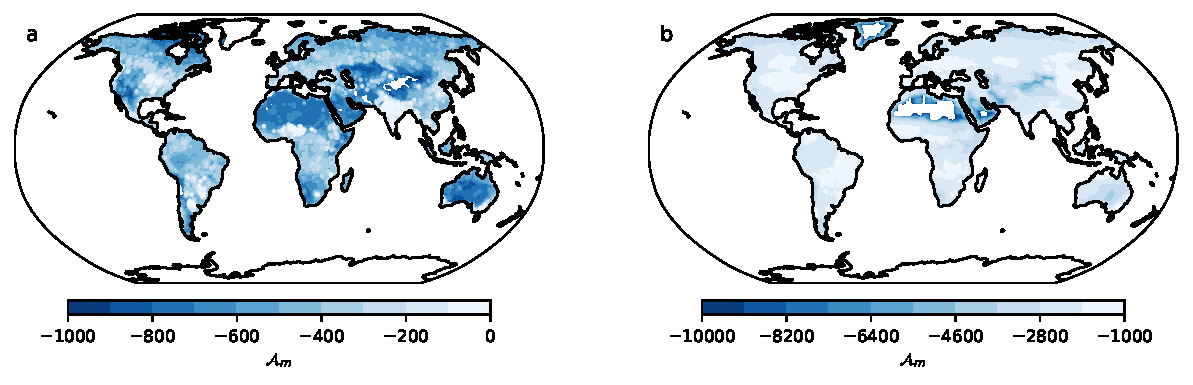
\includegraphics[width=14cm]{Figures/Amin.pdf} % requires the graphicx package
   \caption{Minimum distances ($\mathcal{A}_m$) between (a) NEP from CMIP6 ESMs and X-BASE, and (b) NBP from CMIP6 ESMs and the Jena CarboScope product. More negative values in darker colors indicate smaller distances (values in logarithmic scale), representing larger similarity between the ESMs and the observational products. Note that the numerical scales between a and b are different.}
   \label{fig:Am}
\end{figure}

%\textcolor{blue}{The considerable difference between the NEP and the NBP reference is also evident for the weights of each model (Figures~\ref{fig:wFluxcom} and \ref{fig:wCarboScope}), demonstrating that model weights may change substantially depending on the observational product being used as a reference.}
The weights obtained for each model provide a relative ranking of the models with respect to their distance to the observational product, and serve as a suitable metric to assess model performance. 
The values obtained differed considerably between the NEP and the NBP reference (Figures~\ref{fig:wFluxcom} and \ref{fig:wCarboScope}), which shows that model weights may change substantially depending on the observational product being used as a reference.
Furthermore, for each model, it is clear that there are regions that perform better or worse than others in comparison to the observational product. For example, the MPI-ESM1-2-LR model performs consistently poorly in the Amazon region, in tropical Africa and North America, but performs relatively well in Europe and northern Eurasia. Other models also show consistent spatial patterns of good or poor performance, indicating that the weights do not capture randomly spaced grid-cells, but aggregated regions where the models tend to perform consistently in either direction with respect to the observations. 
These maps of weights also show that there is no one single model that performs best everywhere, or contrastingly, one single model that performs worse everywhere. 

\clearpage 

\begin{figure}[htbp]
   \centering
   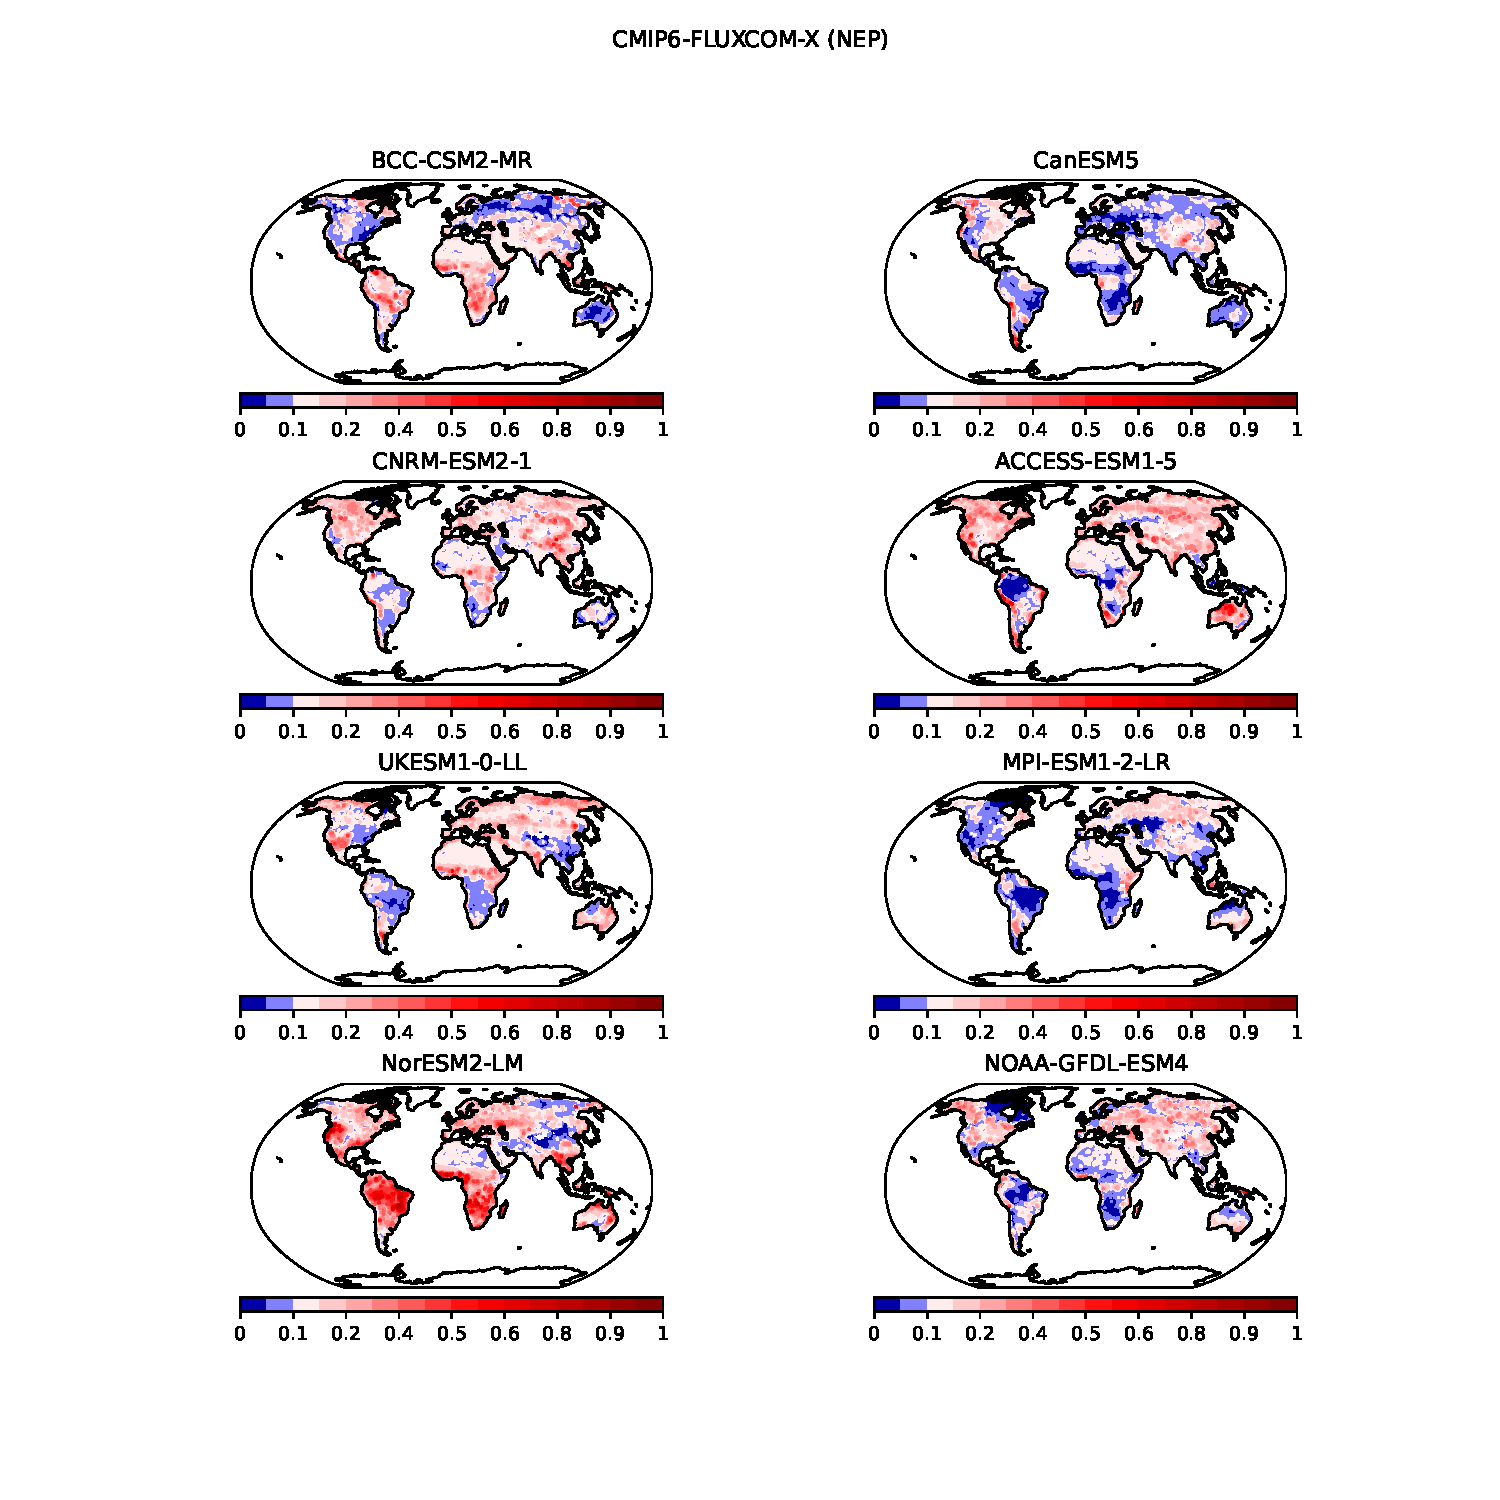
\includegraphics[width=14cm, trim={3cm, 1cm, 2.5cm, 1cm}, clip]{Figures/CMIP6_FLUXCOM_weights.pdf} % requires the graphicx package
   \caption{Weights $w$ of CMIP6 models for the variable NEP with respect to the X-BASE observational product. The diverging color palette is centered at a value of 1/8,  indicating whether a model contributes more or less than the equal weight of 1/8 from the $k= 8$ models. For each grid cell, the sum of the weights of the 8 models adds up to 1. }
   \label{fig:wFluxcom}
\end{figure}

\begin{figure}[htbp]
   \centering
   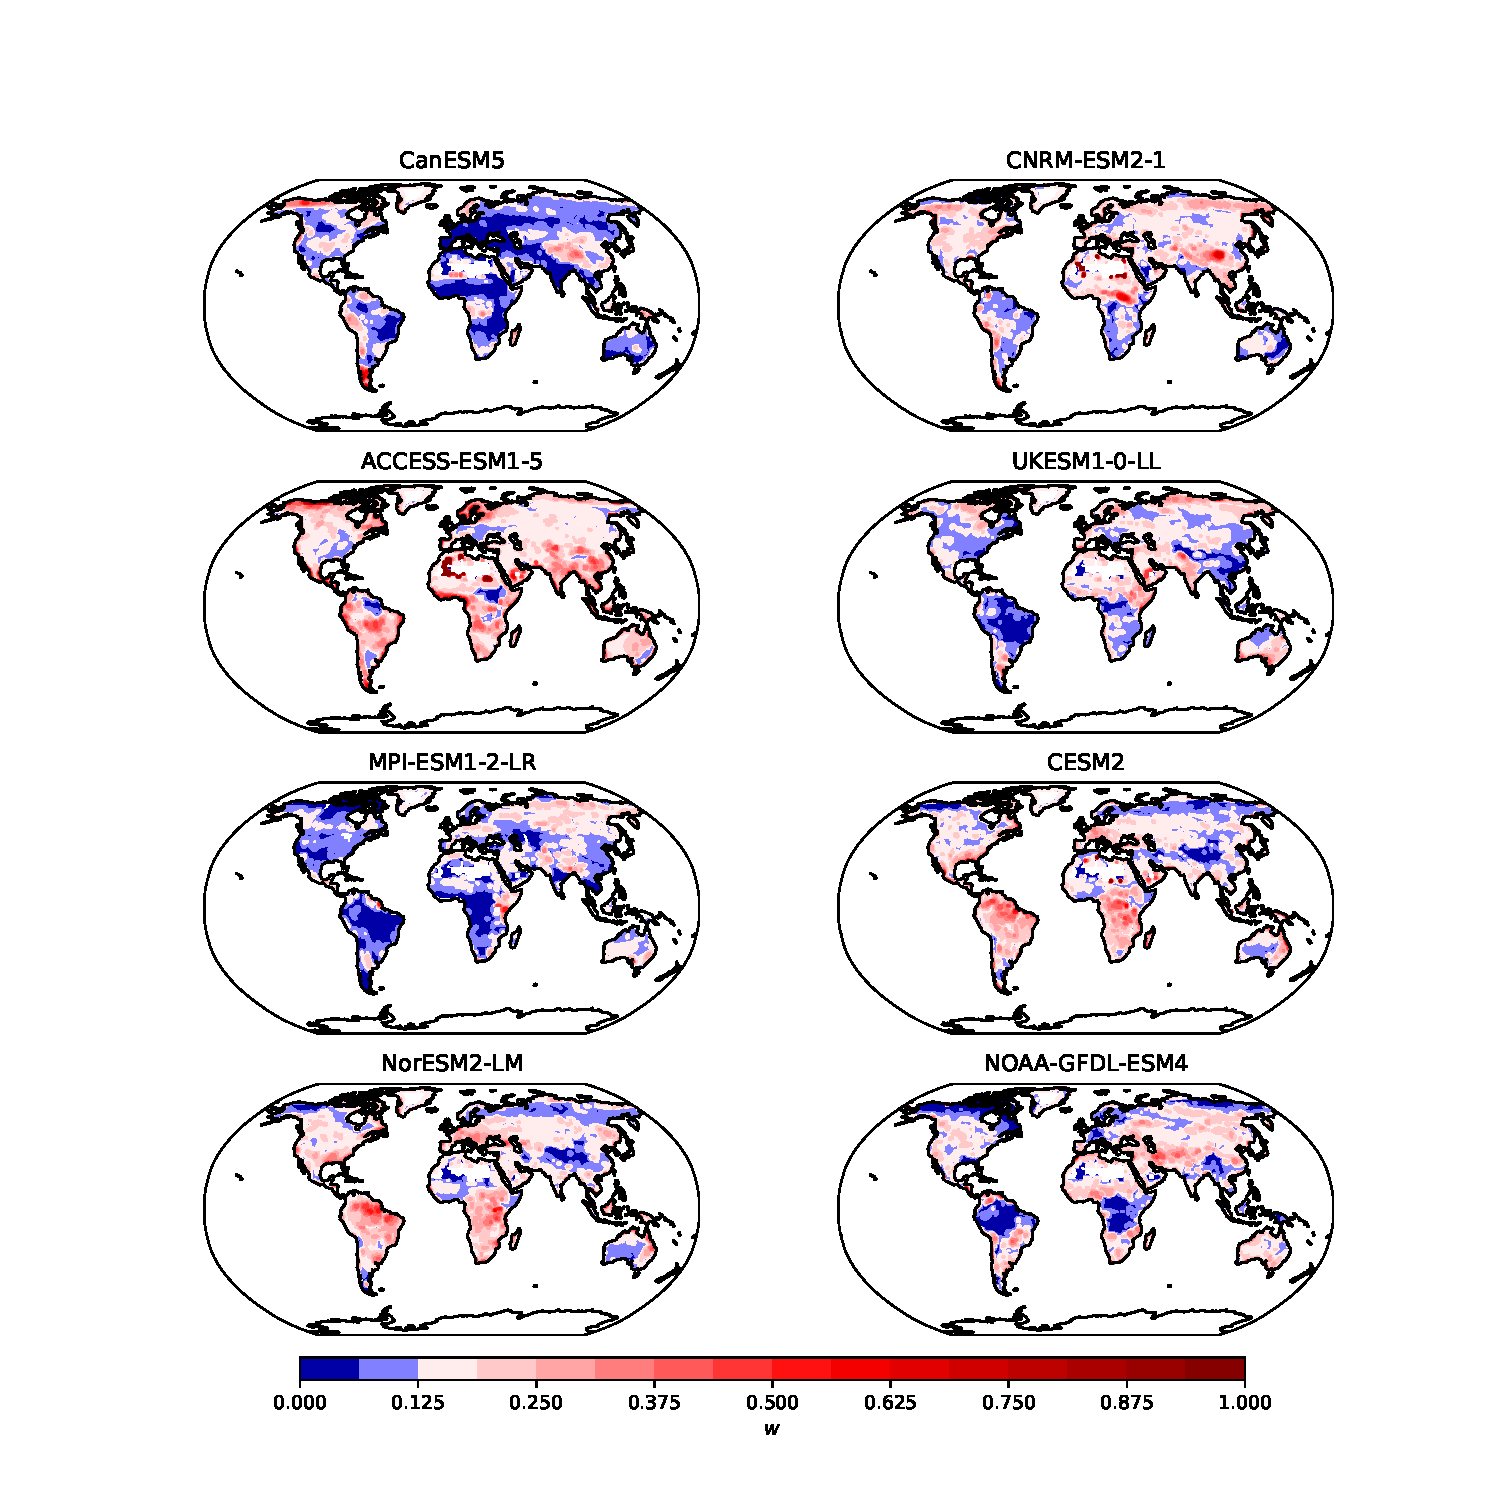
\includegraphics[width=14cm, trim={3cm, 1cm, 2.5cm, 1cm}, clip]{Figures/CMIP6_CarboScope_weights.pdf} % requires the graphicx package
   \caption{Weights $w$ of CMIP6 models for the variable NBP with respect to the Jena CarboScope observational product. The diverging color palette is centered at a value of 1/8,  indicating whether a model contributes more or less than the equal weight of 1/8 from the $k= 8$ models. For each grid cell, the sum of the weights of the 8 models adds up to 1. }
   \label{fig:wCarboScope}
\end{figure}

\clearpage

The values of weights for each grid cell were combined with the predictions of the variable of interest for each model to produce weighted averages at the grid cell level for each time step, and then summed across grid cells to obtain time series (Figure~\ref{fig:averages}).
The obtained results show that the weighted average of NEP  is consistently lower than the arithmetic average, mostly because the influence of models that make predictions with values much higher than the observational product have much less weight in the weighted average (Figure~\ref{fig:averages}a). In fact, the models that predict the highest values of NEP, namely NOAA-GFDL-ESM4 and ACESS-ESM1-5, make predictions well outside the uncertainty range obtained for the weighted average, indicating the small contribution that these models make to the obtained average. 

For the variable NBP, the arithmetic and the weighted average are relatively close to each other for the entire simulation period (Figure~\ref{fig:averages}b). In this case, most models make predictions close to each other and, therefore, they contribute more evenly to the weighted average. Nevertheless, the obtained uncertainty range is lower for the weighted average, indicating that those models closer to the observational product have more weight in terms of both the average and its variance, and therefore help to reduce overall uncertainty in the predictions. 

%This is to be expected because the computed weight tends to be very different for the different models and for specific geographic regions. In fact, we believe this is a major strength of the proposed approach, because the weights are not applied uniformly to all grid cells of a specific model, but according to how these grid cells perform with respect to the observations. 

\begin{figure}[t]
   \centering
   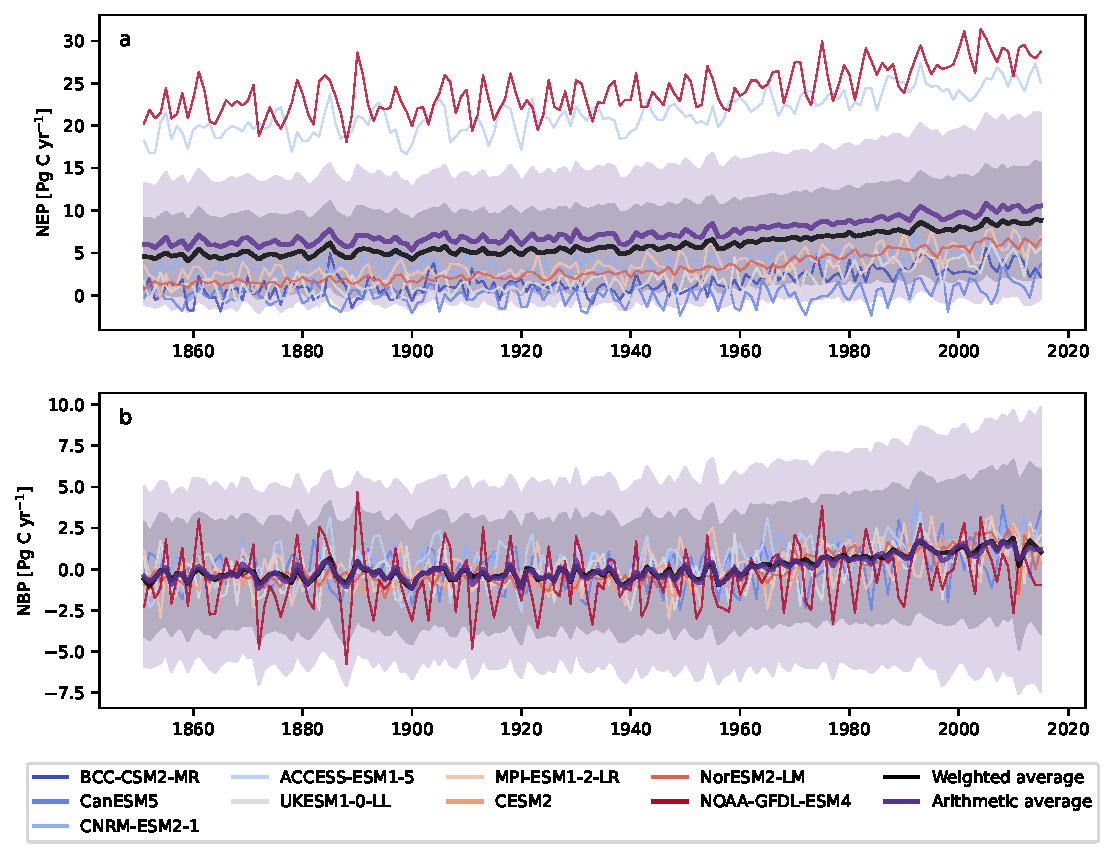
\includegraphics[width=14cm]{Figures/Time_series_NXP_c1.pdf} % requires the graphicx package
   \caption{Annual time series of (a) NEP and (b) NBP from individual CMIP6 ESMs obtained as arithmetic averages (purple lines) and the weighted averages using the method proposed here (black lines). Uncertainty ranges are expressed as the average value $\pm$ the value of $\sigma$ including only the first term from equation \ref{eq:sigma2}. For the arithmetic average, the weights for the computation of uncertainty are $w_i = 1/8$.}
   \label{fig:averages}
\end{figure}

For both variables, NEP and NBP, the estimate of uncertainty with our proposed approach is also significantly lower than the uncertainty based on equal weights (Figures~\ref{fig:averages} and \ref{fig:averagesFullUncertainty}). We obtained a much lower level of uncertainty for the weighted average because the method applies probabilities or strengths of belief to the different models and grid cells, and therefore this averaging procedure increases confidence in the inferred multi-model average. 

However, Figure~\ref{fig:averages} only shows the first component of the variance from equation \ref{eq:sigma2}; i.e., only the deviation of the models with respect to the averages excluding the deviation of the models from the observational product. When combining both sources of uncertainty, the overall variance is much larger, but the uncertainty of the weighted average is still consistently lower than that of the arithmetic average (Figure~\ref{fig:averagesFullUncertainty}). 

It is also important to note that even though the observational products are only available for a short period of time, we used the obtained weights for the entire period of the simulations of the ESMs under the assumption that a model that performs well during the period in which observations are available, should be able to perform well for other periods. This assumption is obviously questionable, and probably inadequate for periods of time much beyond the time range of available data. However, we still believe that this assumption is better than to assume that all models are equally reliable for all periods of time as it is implicitly assumed with an equal weight approach. 

\section{Discussion}
Although other authors have proposed methods to obtain weights and multi-model averages from the predictions of ESMs \citep[and references therein]{Tebaldi2007}, we presented here an approach based on information-theoretic concepts that is easy to implement and can help to improve inferences from ESMs minimizing biases and reducing uncertainties. 
Some of the advantages of this method over others include: (1) a theoretical foundation based on concepts from probability and information theory \citep{Akaike1974, Akaike1981, Anderson2007, Burnham2002}. (2) The weights have a relevant interpretation, they are evidence in favor of a model prediction having the smallest distance to full reality, even though comparisons are only performed with respect to an uncertain observational product. 
(3) Calculation of weights based on spatial performance of model output with respect to observations, and not a uniform weight for all grid-cells of a model.

However, as with other approaches, some weaknesses should be acknowledged and should be improved in future research. These are: first, lack of a log-likelihood function for the assessment of model-observation distances. Although such a function would be unrealistic to obtain given the process of development and parameterization of ESMs, it is still desirable to obtain an unbiased estimator of the log-likelihood of a parameterized model with respect to available data. We are not aware of another method that could be used to replace the simple log of square residuals used here, but it is also important to point out that other measures of distance used in other methods apply mostly the squared residuals as a distance metric. Therefore, our method offers a small theoretical improvement over previous approaches based on the theoretical knowledge that, under certain assumptions, the logarithm of square residuals is a first-order approximation to a maximum likelihood estimator. 

Second, other authors have raised concerns over the issue of model independence \citep{Knutti2010CC, Knutti2010JC}, a problem that we do not address explicitly here. They argue that many models share the same base code or are based on the same underlying principles, and cannot be treated as completely independent estimates for obtaining an unbiased average. In particular, the method of \citet{Knutti2017} produces weights that penalize a model according to its prediction distance to that of other models. We think this is a valid concern, particularly when weights are obtained for the aggregated (sums or averages) across all grid cells of a model. However, the implementation of similar processes in two models but with differences in other components such as its climate sensitivity may lead to very different predictions. For instance, CESM2 and NorESM2-LM share the same land vegetation model, CLM5 (Table~\ref{tab:models}). Although the spatial distribution of the weights for NBP with these models tends to correlate well, the correlation is not uniform across all grid cells and is mostly below 90\% (Figure~\ref{fig:corr}). This implies that a shared component of a model can interact with other non-shared components of each model, resulting in different predictions that should be treated differently for the calculation of weights. 

\begin{figure}[t]
   \centering
   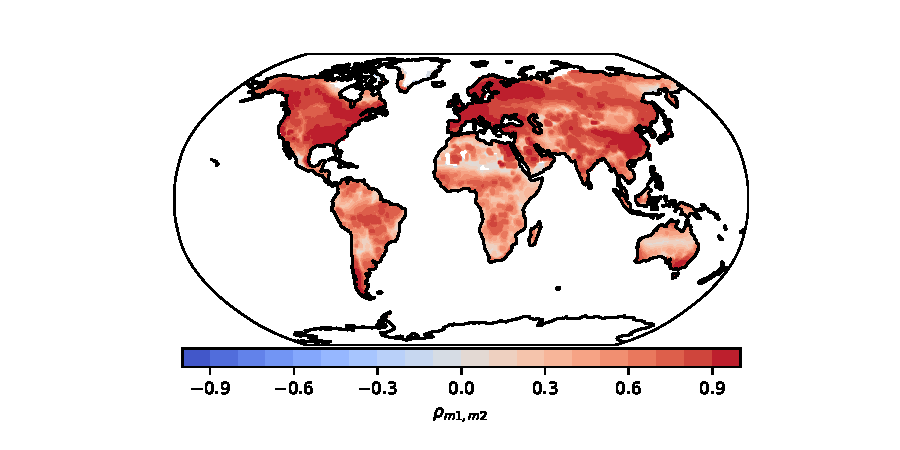
\includegraphics[width=14cm]{Figures/Corr_CESM_NorESM.pdf} % requires the graphicx package
   \caption{Pearson correlation coefficients $\rho$ of variable NBP between CESM2 ($m1$) and NorESM-LM ($m2$). These two models share the same land model (CLM5), but due to differences in other components of the model, the predictions of NBP are not similar and often correlate with values of $\rho < 0.9$.}
   \label{fig:corr}
\end{figure}


It is also important to note that, in the ideal case in which we would have a perfect understanding of Earth system processes, all mathematical models representing these processes would converge to the same predictions. Therefore, it is still debatable whether models that agree with each other because they have a common representation of underlying processes should be penalized. For this reason, we refrain from introducing a penalization term to our computation of weights, but we acknowledge that this is an issue that deserves more theoretical work. 

A third issue that deserves more attention is the lack of penalization for model complexity in the approach we propose. The original work proposed by H. Akaike is very well known for the introduction of a penalization term due to the number of parameters in the model, a penalization well supported by mathematical theory and philosophy of science \citep{Akaike1974, Akaike1981}. However, the scientific trend in ESM development is the addition of increased levels of detail supported by increased computational power \citep{Held2005, Held2014}. We do not have information on the total number of parameters used in each ESM, but we believe it should be on the order of $10^2$ -- $10^3$. Therefore, adding a penalization term as in the traditional form in the computation of AIC would lead to differences among models that are dominated by differences in their number of parameters, obscuring differences in model distances with respect to observations. But ignoring the penalization due to model complexity, as we do in our approach, implies that we continue ignoring the tension between model complexity and understanding, and focus exclusively on model performance. We believe this a topic that deserves much more theoretical attention and should be addressed in future improvements on the approach we propose. 


\conclusions  %% \conclusions[modified heading if necessary]
We proposed here an approach to obtain probabilities of model performance with respect to available observational products, and to derive weights of evidence in favor of a model being the best from a set of available models. These weights are not constants for a particular model, but are obtained at the grid-cell level for each model. They provide estimates of the relative likelihood that a model performs well at a particular grid cell and therefore can be used as the weight of evidence for a model performing well in a particular location. We believe this probabilistic interpretation, grounded on solid concepts from information theory, provides advantages over other methods and can be of real practical use for making inferences of average behavior in Earth system science. 

Using this approach for obtaining ensemble averages of the variables NEP and NBP from models participating in CMIP6, we found that our proposed weights can significantly reduce bias when a small number of models make predictions further away from a reference observational product and all other models in the ensemble. The prediction uncertainty for the weighted average is also smaller than the uncertainty of the arithmetic average. Overall, the approach helps to increase confidence in inferring spatial and temporal behaviors from multiple models.


%% The following commands are for the statements about the availability of data sets and/or software code corresponding to the manuscript.
%% It is strongly recommended to make use of these sections in case data sets and/or software code have been part of your research the article is based on.

%\codeavailability{TEXT} %% use this section when having only software code available


%\dataavailability{TEXT} %% use this section when having only data sets available


\codedataavailability{The exact version of the code used to produce the results used in this article is archived on repository under DOI: 10.5281/zenodo.15167573 \citep{Sierra2025}, as well as the model weights necessary to compute model averages \citep{Sierra2025}.}

%All code to reproduce the results is properly archived at Zenodo \citep[][DOI: 10.5281/zenodo.15167573]{Sierra2025}. Original data from CMIP6 model output was obtained from the German Climate Computing Center (DKRZ), openly available at \url{https://cmip-data-pool.dkrz.de/}.} %% use this section when having data sets and software code available


%\sampleavailability{TEXT} %% use this section when having geoscientific samples available


%\videosupplement{TEXT} %% use this section when having video supplements available

\clearpage

\appendix
\section{Supplementary figures}    %% Appendix A

\begin{figure}[htbp]
   \centering
   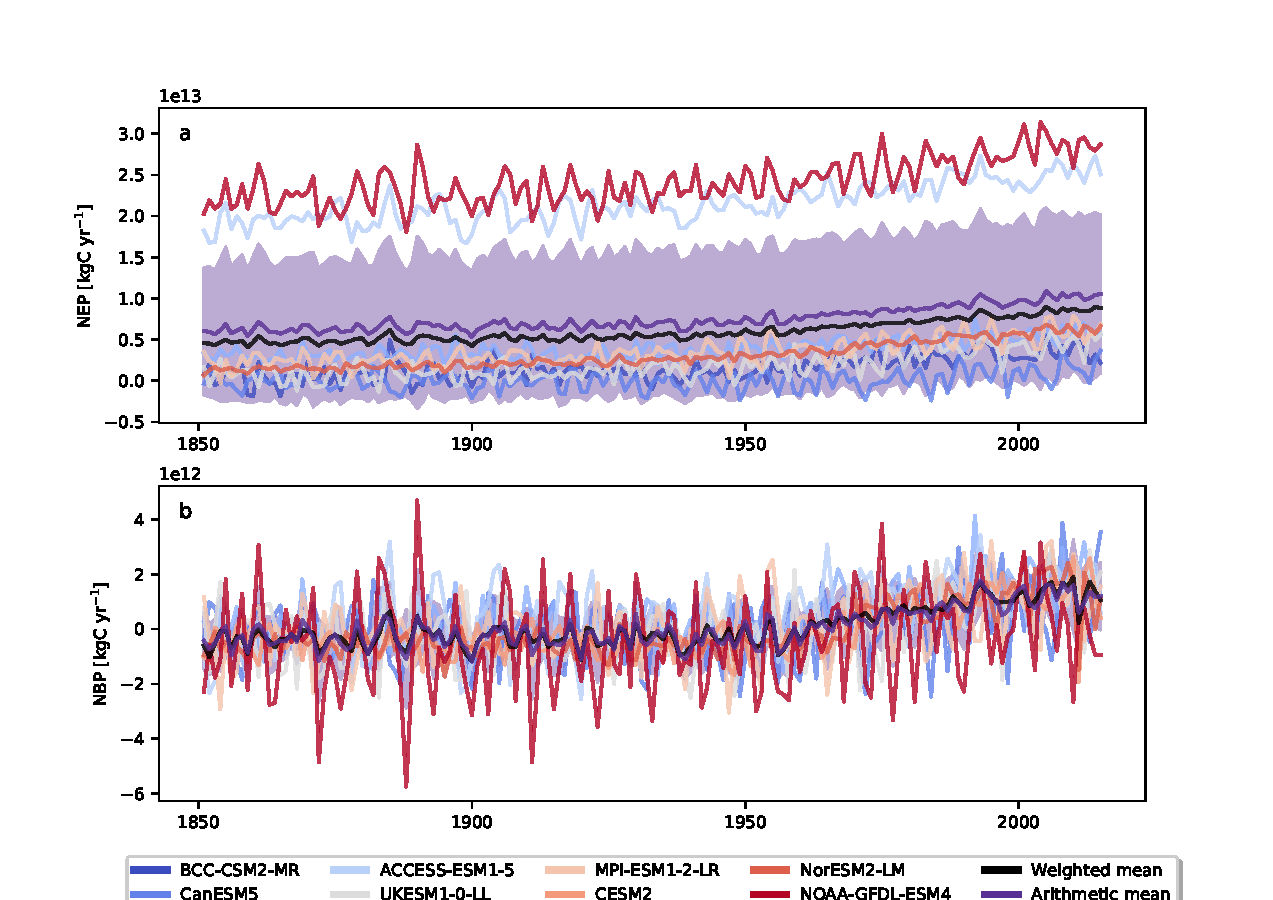
\includegraphics[width=14cm]{Figures/Time_series_NXP.pdf} % requires the graphicx package
   \caption{Annual time series of (a) NEP and (b) NBP from individual CMIP6 ESMs obtained as arithmetic averages (purple lines) and the weighted averages using the method proposed here (black lines). Uncertainty ranges are expressed as the average value $\pm$ the full value of $\sigma$ from equation \ref{eq:sigma2}. For the arithmetic average, the weights for the computation of uncertainty are $w_i = 1/8$.}
   \label{fig:averagesFullUncertainty}
\end{figure}

\begin{figure}[htbp]
   \centering
   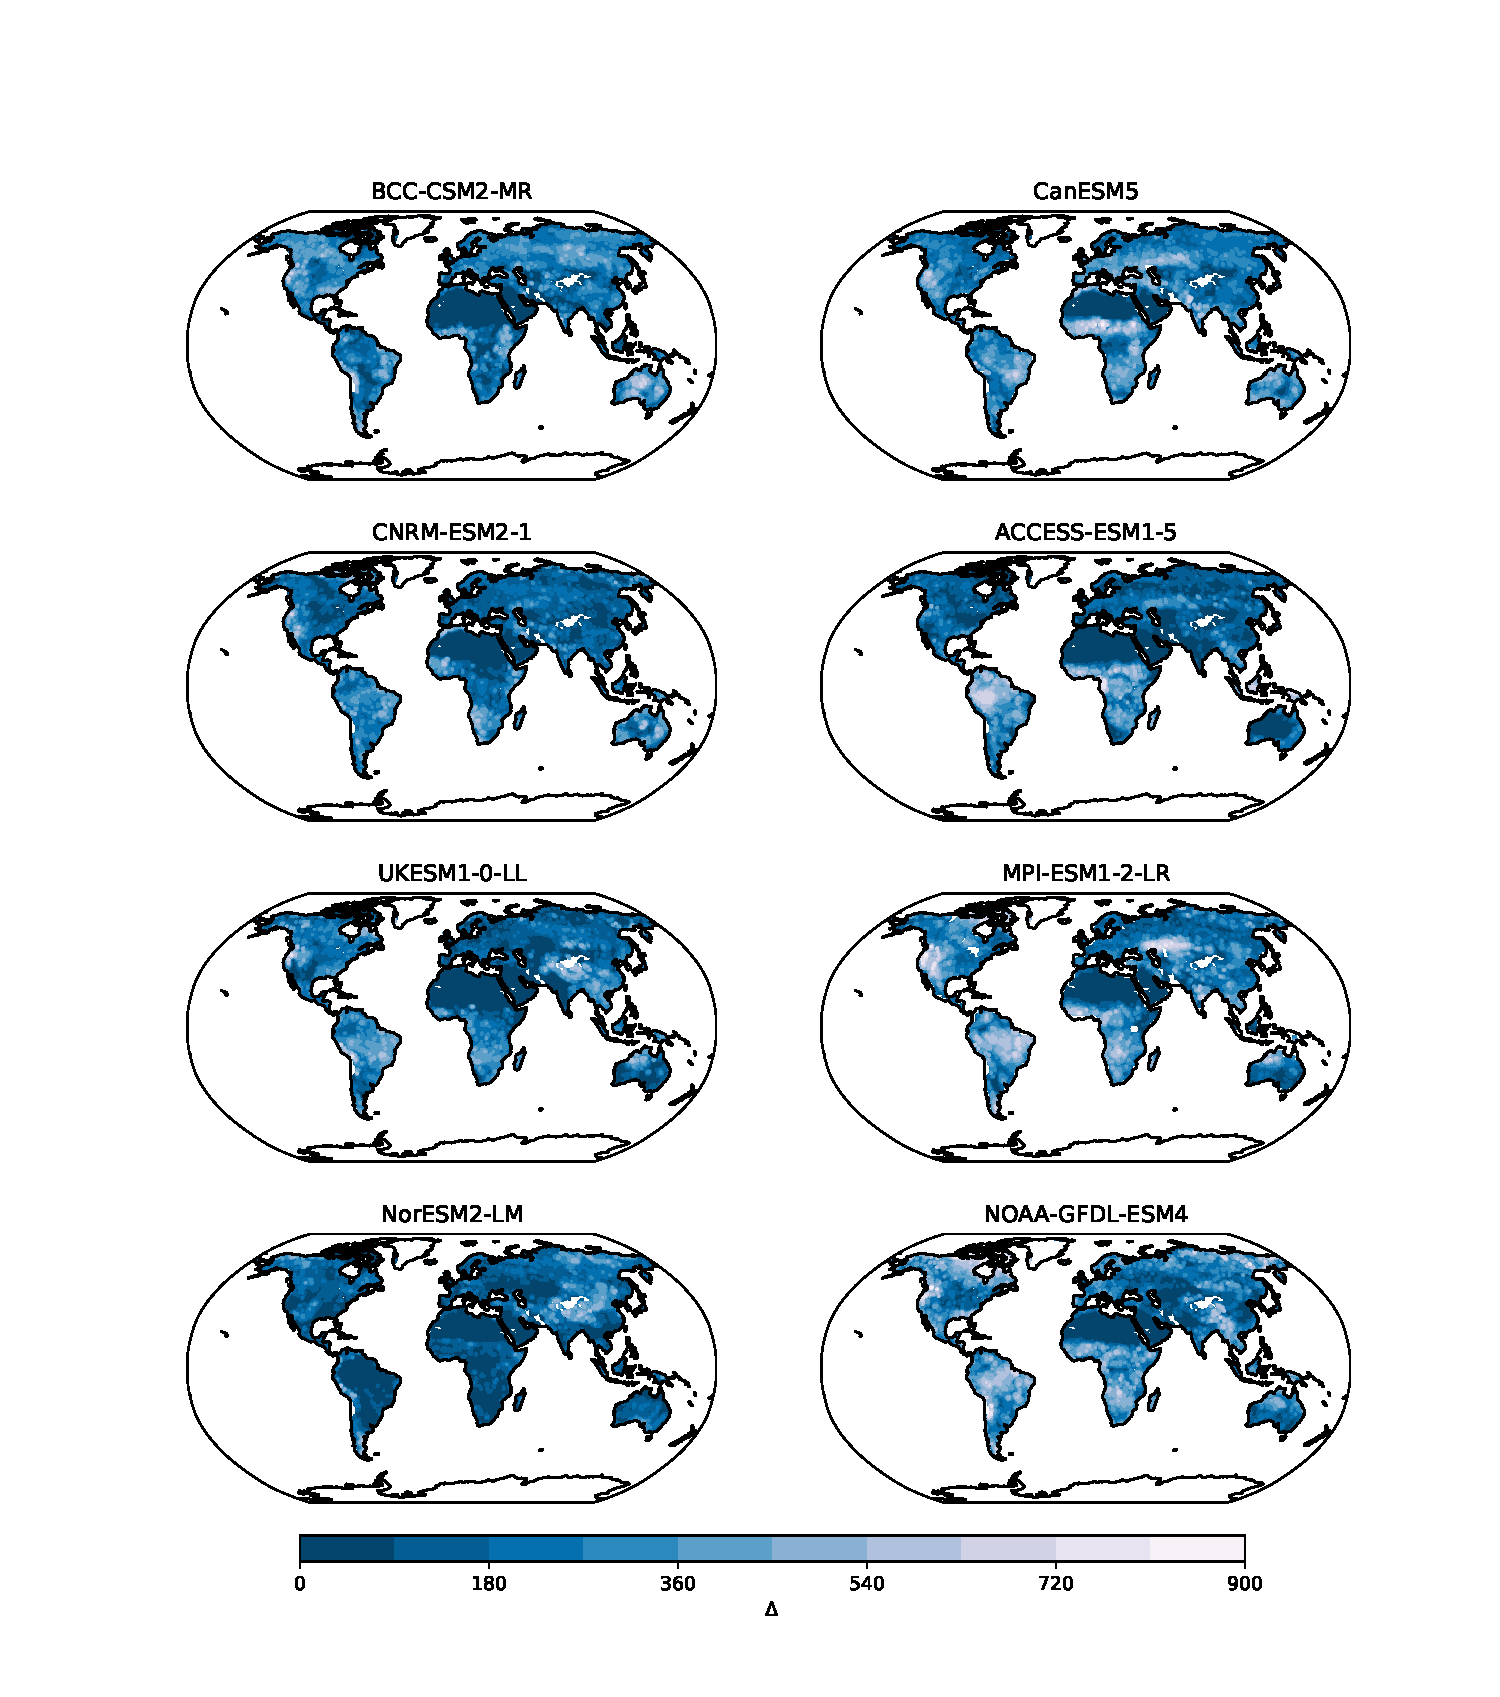
\includegraphics[width=16cm]{Figures/CMIP6_FLUXCOM-X_D.pdf} % requires the graphicx package
   \caption{Maps of differences $\Delta$ with respect to minimum distances ($\mathcal{A}_m$) of CMIP6 models for the variable NEP and the X-BASE observational product. Small numbers in darker colors indicate smaller distances, representing a larger similarity between ESMs and X-BASE.}
   \label{fig:Delta_NEP}
\end{figure}

\begin{figure}[htbp]
   \centering
   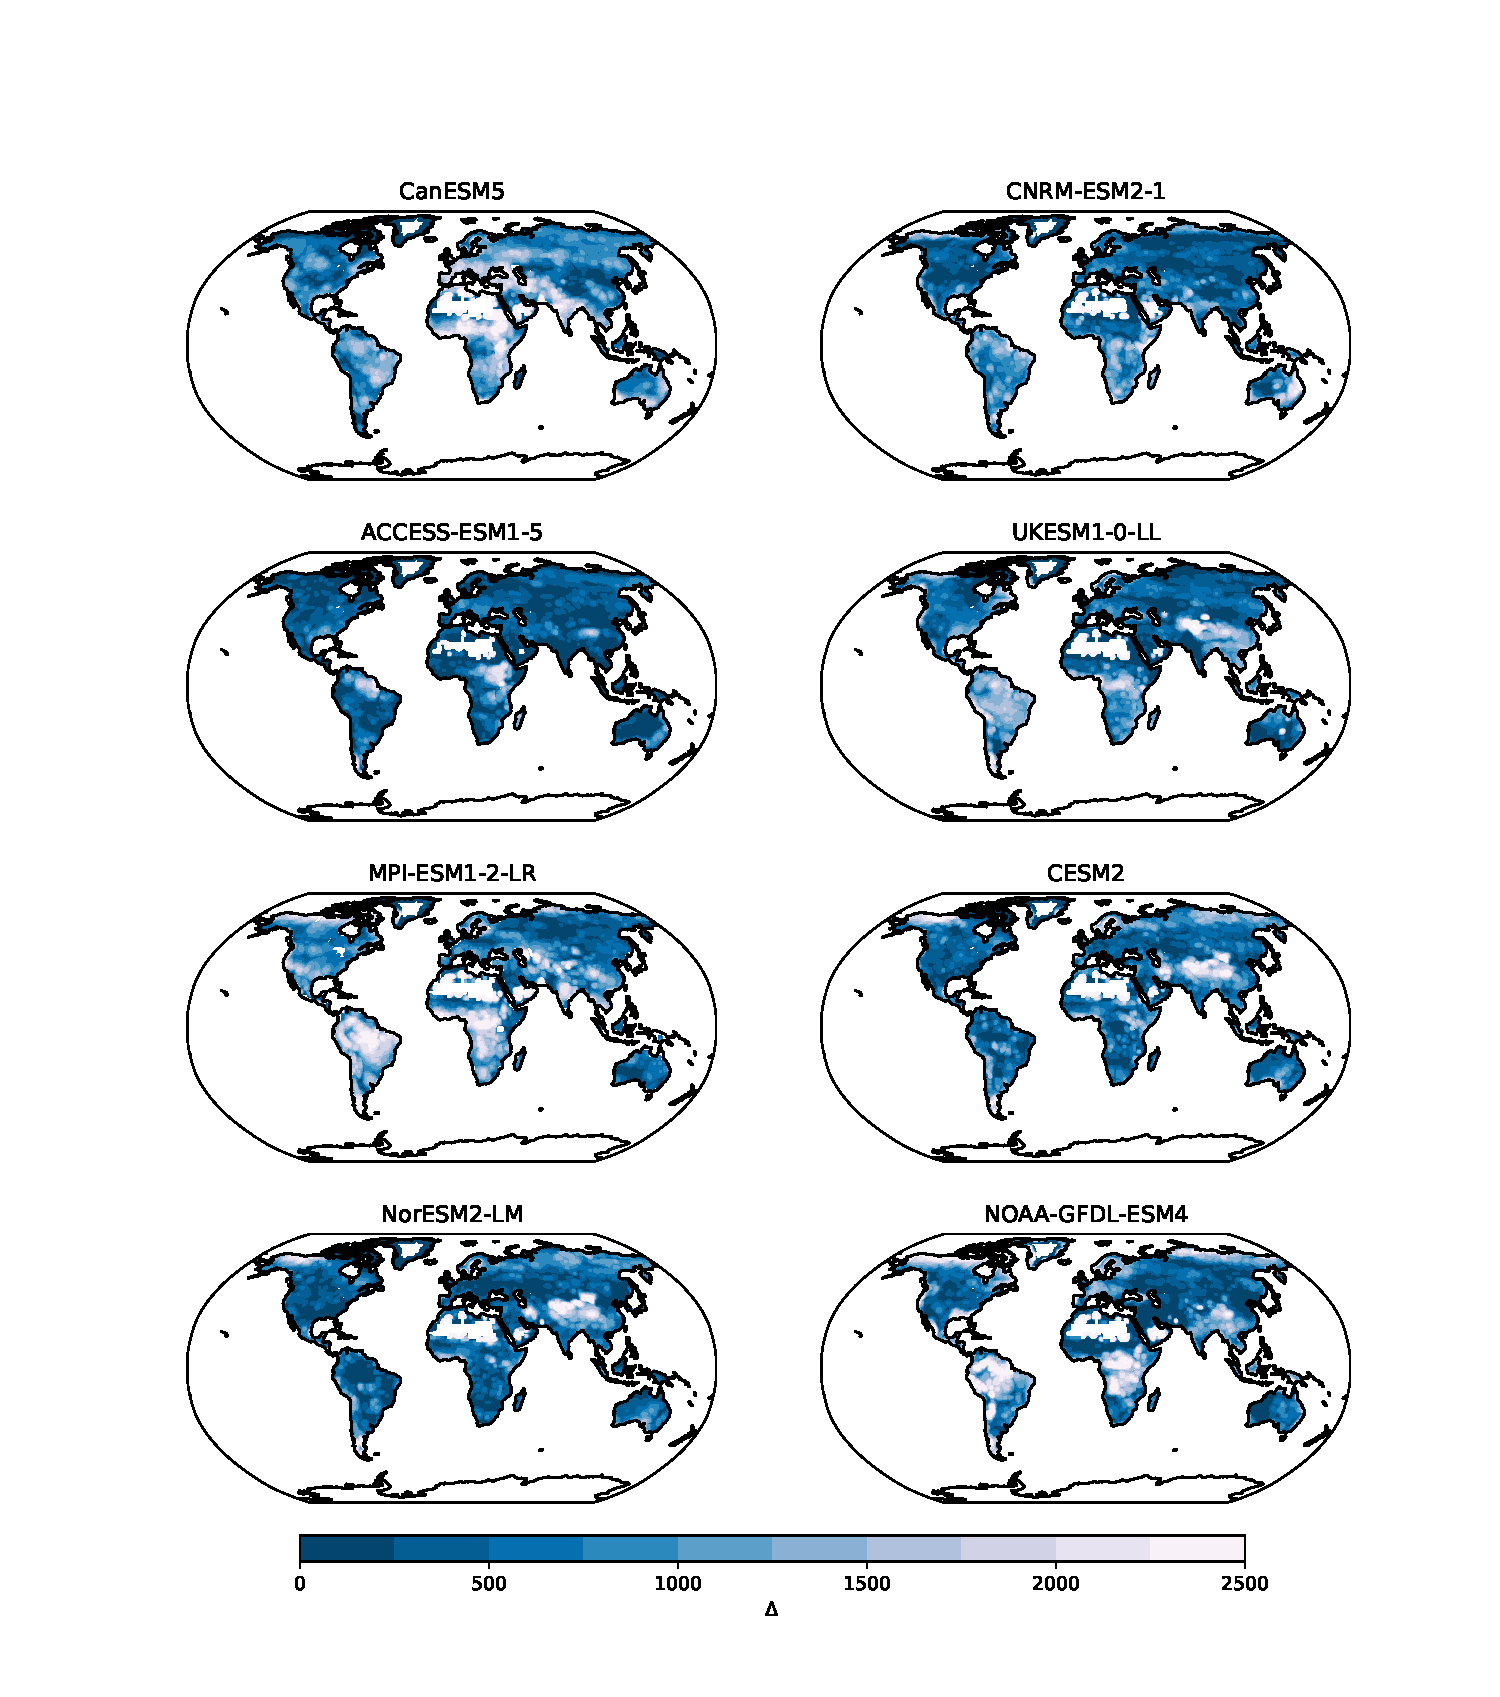
\includegraphics[width=16cm]{Figures/CMIP6_CarboScope_D.pdf} % requires the graphicx package
   \caption{Maps of differences $\Delta$ with respect to minimum distances ($\mathcal{A}_m$) of CMIP6 models for the variable NBP and the Jena CarboScope observational product. Small numbers in darker colors indicate smaller distances, representing a larger similarity between ESMs and CarboScope.}
   \label{fig:Delta_NBP}
\end{figure}

%\subsection{}     %% Appendix A1, A2, etc.


\noappendix       %% use this to mark the end of the appendix section. Otherwise the figures might be numbered incorrectly (e.g. 10 instead of 1).

%% Regarding figures and tables in appendices, the following two options are possible depending on your general handling of figures and tables in the manuscript environment:

%% Option 1: If you sorted all figures and tables into the sections of the text, please also sort the appendix figures and appendix tables into the respective appendix sections.
%% They will be correctly named automatically.

%% Option 2: If you put all figures after the reference list, please insert appendix tables and figures after the normal tables and figures.
%% To rename them correctly to A1, A2, etc., please add the following commands in front of them:

\appendixfigures  %% needs to be added in front of appendix figures

\appendixtables   %% needs to be added in front of appendix tables

%% Please add \clearpage between each table and/or figure. Further guidelines on figures and tables can be found below.

\clearpage

\authorcontribution{CAS: Conceptualization, methodology, writing--original draft. EM: Data curation, investigation, software, visualization, writing--review \& editing.} %% this section is mandatory

%\competinginterests{TEXT} %% this section is mandatory even if you declare that no competing interests are present

%\disclaimer{TEXT} %% optional section

\begin{acknowledgements}
CAS acknowledges core funding from the Max Planck Society. EM received funding from the European Union’s Horizon 2020 research and innovation programme under the Marie Skłodowska Curie grant agreement No 101110350. 
\end{acknowledgements}




%% REFERENCES

%% The reference list is compiled as follows:

%\begin{thebibliography}{}
%
%\bibitem[AUTHOR(YEAR)]{LABEL1}
%REFERENCE 1
%
%\bibitem[AUTHOR(YEAR)]{LABEL2}
%REFERENCE 2
%
%\end{thebibliography}

%% Since the Copernicus LaTeX package includes the BibTeX style file copernicus.bst,
%% authors experienced with BibTeX only have to include the following two lines:
%%
 \bibliographystyle{copernicus}
 \bibliography{refs.bib}
%%
%% URLs and DOIs can be entered in your BibTeX file as:
%%
%% URL = {http://www.xyz.org/~jones/idx_g.htm}
%% DOI = {10.5194/xyz}


%% LITERATURE CITATIONS
%%
%% command                        & example result
%% \citet{jones90}|               & Jones et al. (1990)
%% \citep{jones90}|               & (Jones et al., 1990)
%% \citep{jones90,jones93}|       & (Jones et al., 1990, 1993)
%% \citep[p.~32]{jones90}|        & (Jones et al., 1990, p.~32)
%% \citep[e.g.,][]{jones90}|      & (e.g., Jones et al., 1990)
%% \citep[e.g.,][p.~32]{jones90}| & (e.g., Jones et al., 1990, p.~32)
%% \citeauthor{jones90}|          & Jones et al.
%% \citeyear{jones90}|            & 1990



%% FIGURES

%% When figures and tables are placed at the end of the MS (article in one-column style), please add \clearpage
%% between bibliography and first table and/or figure as well as between each table and/or figure.

% The figure files should be labelled correctly with Arabic numerals (e.g. fig01.jpg, fig02.png).


%% ONE-COLUMN FIGURES

%%f
%\begin{figure}[t]
%\includegraphics[width=8.3cm]{FILE NAME}
%\caption{TEXT}
%\end{figure}
%
%%% TWO-COLUMN FIGURES
%
%%f
%\begin{figure*}[t]
%\includegraphics[width=12cm]{FILE NAME}
%\caption{TEXT}
%\end{figure*}
%
%
%%% TABLES
%%%
%%% The different columns must be seperated with a & command and should
%%% end with \\ to identify the column brake.
%
%%% ONE-COLUMN TABLE
%
%%t
%\begin{table}[t]
%\caption{TEXT}
%\begin{tabular}{column = lcr}
%\tophline
%
%\middlehline
%
%\bottomhline
%\end{tabular}
%\belowtable{} % Table Footnotes
%\end{table}
%
%%% TWO-COLUMN TABLE
%
%%t
%\begin{table*}[t]
%\caption{TEXT}
%\begin{tabular}{column = lcr}
%\tophline
%
%\middlehline
%
%\bottomhline
%\end{tabular}
%\belowtable{} % Table Footnotes
%\end{table*}
%
%%% LANDSCAPE TABLE
%
%%t
%\begin{sidewaystable*}[t]
%\caption{TEXT}
%\begin{tabular}{column = lcr}
%\tophline
%
%\middlehline
%
%\bottomhline
%\end{tabular}
%\belowtable{} % Table Footnotes
%\end{sidewaystable*}
%
%
%%% MATHEMATICAL EXPRESSIONS
%
%%% All papers typeset by Copernicus Publications follow the math typesetting regulations
%%% given by the IUPAC Green Book (IUPAC: Quantities, Units and Symbols in Physical Chemistry,
%%% 2nd Edn., Blackwell Science, available at: http://old.iupac.org/publications/books/gbook/green_book_2ed.pdf, 1993).
%%%
%%% Physical quantities/variables are typeset in italic font (t for time, T for Temperature)
%%% Indices which are not defined are typeset in italic font (x, y, z, a, b, c)
%%% Items/objects which are defined are typeset in roman font (Car A, Car B)
%%% Descriptions/specifications which are defined by itself are typeset in roman font (abs, rel, ref, tot, net, ice)
%%% Abbreviations from 2 letters are typeset in roman font (RH, LAI)
%%% Vectors are identified in bold italic font using \vec{x}
%%% Matrices are identified in bold roman font
%%% Multiplication signs are typeset using the LaTeX commands \times (for vector products, grids, and exponential notations) or \cdot
%%% The character * should not be applied as mutliplication sign
%
%
%%% EQUATIONS
%
%%% Single-row equation
%
%\begin{equation}
%
%\end{equation}
%
%%% Multiline equation
%
%\begin{align}
%& 3 + 5 = 8\\
%& 3 + 5 = 8\\
%& 3 + 5 = 8
%\end{align}
%
%
%%% MATRICES
%
%\begin{matrix}
%x & y & z\\
%x & y & z\\
%x & y & z\\
%\end{matrix}
%
%
%%% ALGORITHM
%
%\begin{algorithm}
%\caption{...}
%\label{a1}
%\begin{algorithmic}
%...
%\end{algorithmic}
%\end{algorithm}
%
%
%%% CHEMICAL FORMULAS AND REACTIONS
%
%%% For formulas embedded in the text, please use \chem{}
%
%%% The reaction environment creates labels including the letter R, i.e. (R1), (R2), etc.
%
%\begin{reaction}
%%% \rightarrow should be used for normal (one-way) chemical reactions
%%% \rightleftharpoons should be used for equilibria
%%% \leftrightarrow should be used for resonance structures
%\end{reaction}
%
%
%%% PHYSICAL UNITS
%%%
%%% Please use \unit{} and apply the exponential notation


\end{document}
